\subsection{The Challenges: Foregrounds and Systematics}
\label{sec:foregrounds}
\vspace{-0.05in}

A minimum target for the CMB Probe is to constrain the tensor to scalar ratio with $\sigma(r) < 0.001$. Data from \planck\ and 
sub-orbital experiments reveal that incomplete knowledge of the polarized foregrounds currently limits the measurements. 
Reducing $r$ uncertainties from their current $0.1$ level will have to be accompanied by equivalent higher fidelity measurements of the foregrounds. 



A satellite mission provides a unique opportunity to target both the inflationary B-mode polarization that originates from the epoch of recombination and peaks around $\ell=80$ and the contribution that peaks on significantly larger scales $\ell\lesssim 12$. To measure the contribution from reionization will require an unprecedented understanding of foregrounds and systematic effects. This is illustrated in the left panel of Figure~\ref{fig:Qrp001}, which shows the contribution from reionization to the Stokes $Q$-parameter for $r=0.001$. The amplitude of the signal is approximately $10$ nK

%A satellite experiment enables
%full-sky observations, and provides 

The CMB Probe has complete flexibility in the choice of frequency coverage, both of which are challenging from the ground or from the balloon platform.  Among other limitations, the atmosphere prevents observations at key frequencies, such as 60\,GHz, and requires data filtering that makes it difficult to recover the larger angular scales.

By the time a probe-class mission launches, substantial progress will
have been made in this quest.  In the absence of a primordial $B$-mode
signal at detectable levels, the mission will significantly improve
the upper limit on the tensor-to-scalar ratio $r$, with
$\sigma(r)\!\sim\!10^{-3}$.  However, if $r$ is large enough,
tentative $B$-mode detections could be reported from the ground or by
ballon experiments ahead of this mission. The significance of such a
discovery would be such that the detailed characterization of the
angular and spectral dependence of the signal, as well as the
verification of its isotropy across the sky, both of which are
uniquely enabled by a satellite mission, would be required to confirm
its primordial origin \comred{(cite Decadal Survey)}.

In this scenario, a probe-class mission will in particular detect and
characterize the reionization signal expected at the largest angular
scales (multipoles below $\sim\!10$), where observations from other
platforms are the most challenging. The contribution from reionization
to the Stokes parameter $Q$ for $r=0.001$ is shown in the left panel
of Figure~\ref{fig:Qrp001}. The amplitude of this signal is
$\sim\!10$\,nK, which requires that any experiment attempting to
measure it control large-scale foregrounds and systematics at the
unprecedented level of a few nK.

\begin{figure}[h]
\begin{center}
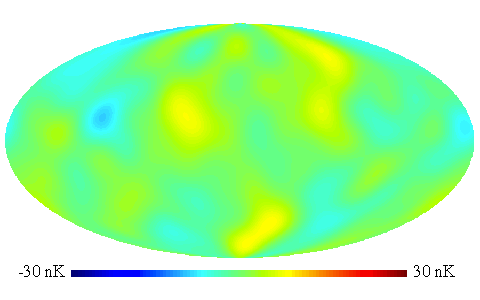
\includegraphics[width=3.2in]{Figures/P15_2_12_rp001.pdf}
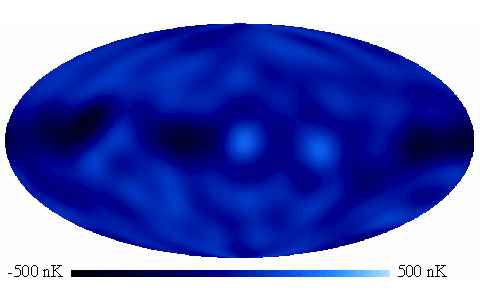
\includegraphics[width=3.2in]{Figures/P353_N_2_12.pdf}
\end{center}
\caption{{\it Left panel:} Contribution to the Stokes $Q$ parameter
  from inflationary $B$-modes for $\ell<12$ and $r=0.001$. {\it Right
    panel:} Noise in the $Planck$ 353 GHz map of the Stokes $Q$
  parameter for $\ell<12$ rescaled to 150\,GHz assuming the spectral
  properties of dust.}
\label{fig:Qrp001}
\end{figure}

\subsubsection{Foregrounds}

Data from the \emph{Planck} satellite have significantly improved our
understanding of foregrounds in both intensity and polarization.
 %In intensity, $Planck$, for example, showed the unexpected relevance of Carbon-Monoxide lines at moderate latitudes as well as the existence of an anomalous emission from dust at low frequencies.
In polarization, the sky is dominated by emission 
of dust grains and synchrotron radiation. \planck\ has provided us with much
improved measurements of their amplitude and spectral dependence. The
observed frequency spectra of both foregrounds are shown for three sky
fractions in the left panel of Figure~\ref{fig:frequency}.  \emph{Even
  in the cleanest patches of the sky}, polarized foreground emission
is brighter than the sought-after primordial $B$-mode signal by over
an order of magnitude at all frequencies.  This statement holds at all
angular scales relevant to the search for primordial $B$-modes, as
shown in the right panel of Figure~\ref{fig:frequency}.

Perfect knowledge of the foreground components would enable their
removal from microwave data, but the sensitivity of the \emph{Planck}
measurements limits it at a level insufficient to detect primordial
$B$-modes, even for values of $r\!\sim\!10^{-1}$. The right panel of
Figure~\ref{fig:Qrp001} shows the noise in the \emph{Planck} 353\,GHz
map of the Stokes $Q$ parameter at the angular scales relevant for
primordial $B$-mode measurements, and rescaled to 150\,GHz assuming
the spectral dependence of dust; it is over an order of magnitude
larger than the inflationary contribution for $r=0.001$.  A mission
aiming to detect primordial $B$-modes at this level across the sky
will therefore not be able to rely on existing data. High
signal-to-noise foreground measurements must accompany those at
frequencies where the CMB contribution is larger.  As discussed below,
optimizing the frequency coverage of these measurements will be a key
goal of the mission concept study.

While the search for primordial B-modes leads to the strictest constraints on foreground residuals, exquisit control of foregrounds is also necessary for other science objectives. A satellite mission is likely also the only reliable way to measure the optical depth at a level necessary to break the degeneracy with the neutrino mass. Furthermore, a cosmic variance limited measurement of E-mode polarization on large scales possible with a probe mission would contain valuable information about the star formation history. 

Similarly, a clear objective of the spectral science is to have a robust, foreground-marginalized expectation of detecting the $\mu$-distortion generated by the dissipation of small-scale acoustic modes in $\Lambda$CDM. While an instrument like PIXIE just falls short of this objective, it seems within reach of a probe mission.

\begin{figure}[h]
\begin{center}
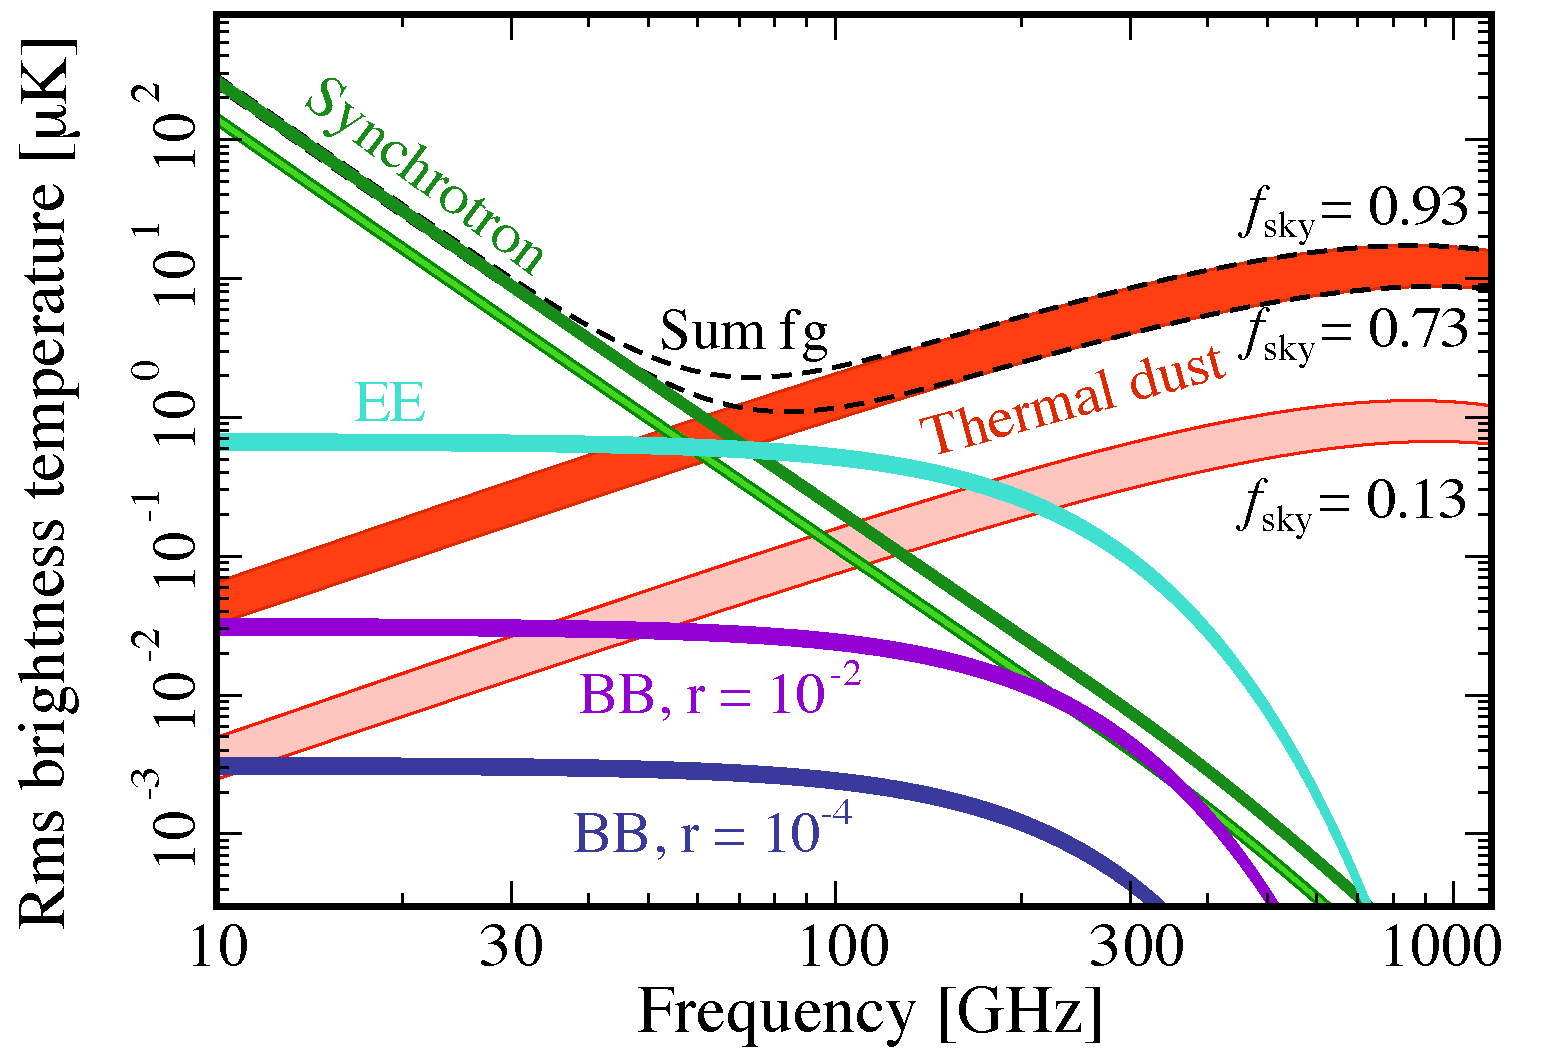
\includegraphics[width=3.26in]{Figures/overview_pol_v4_fsky_noplanck.pdf}\hskip .2cm
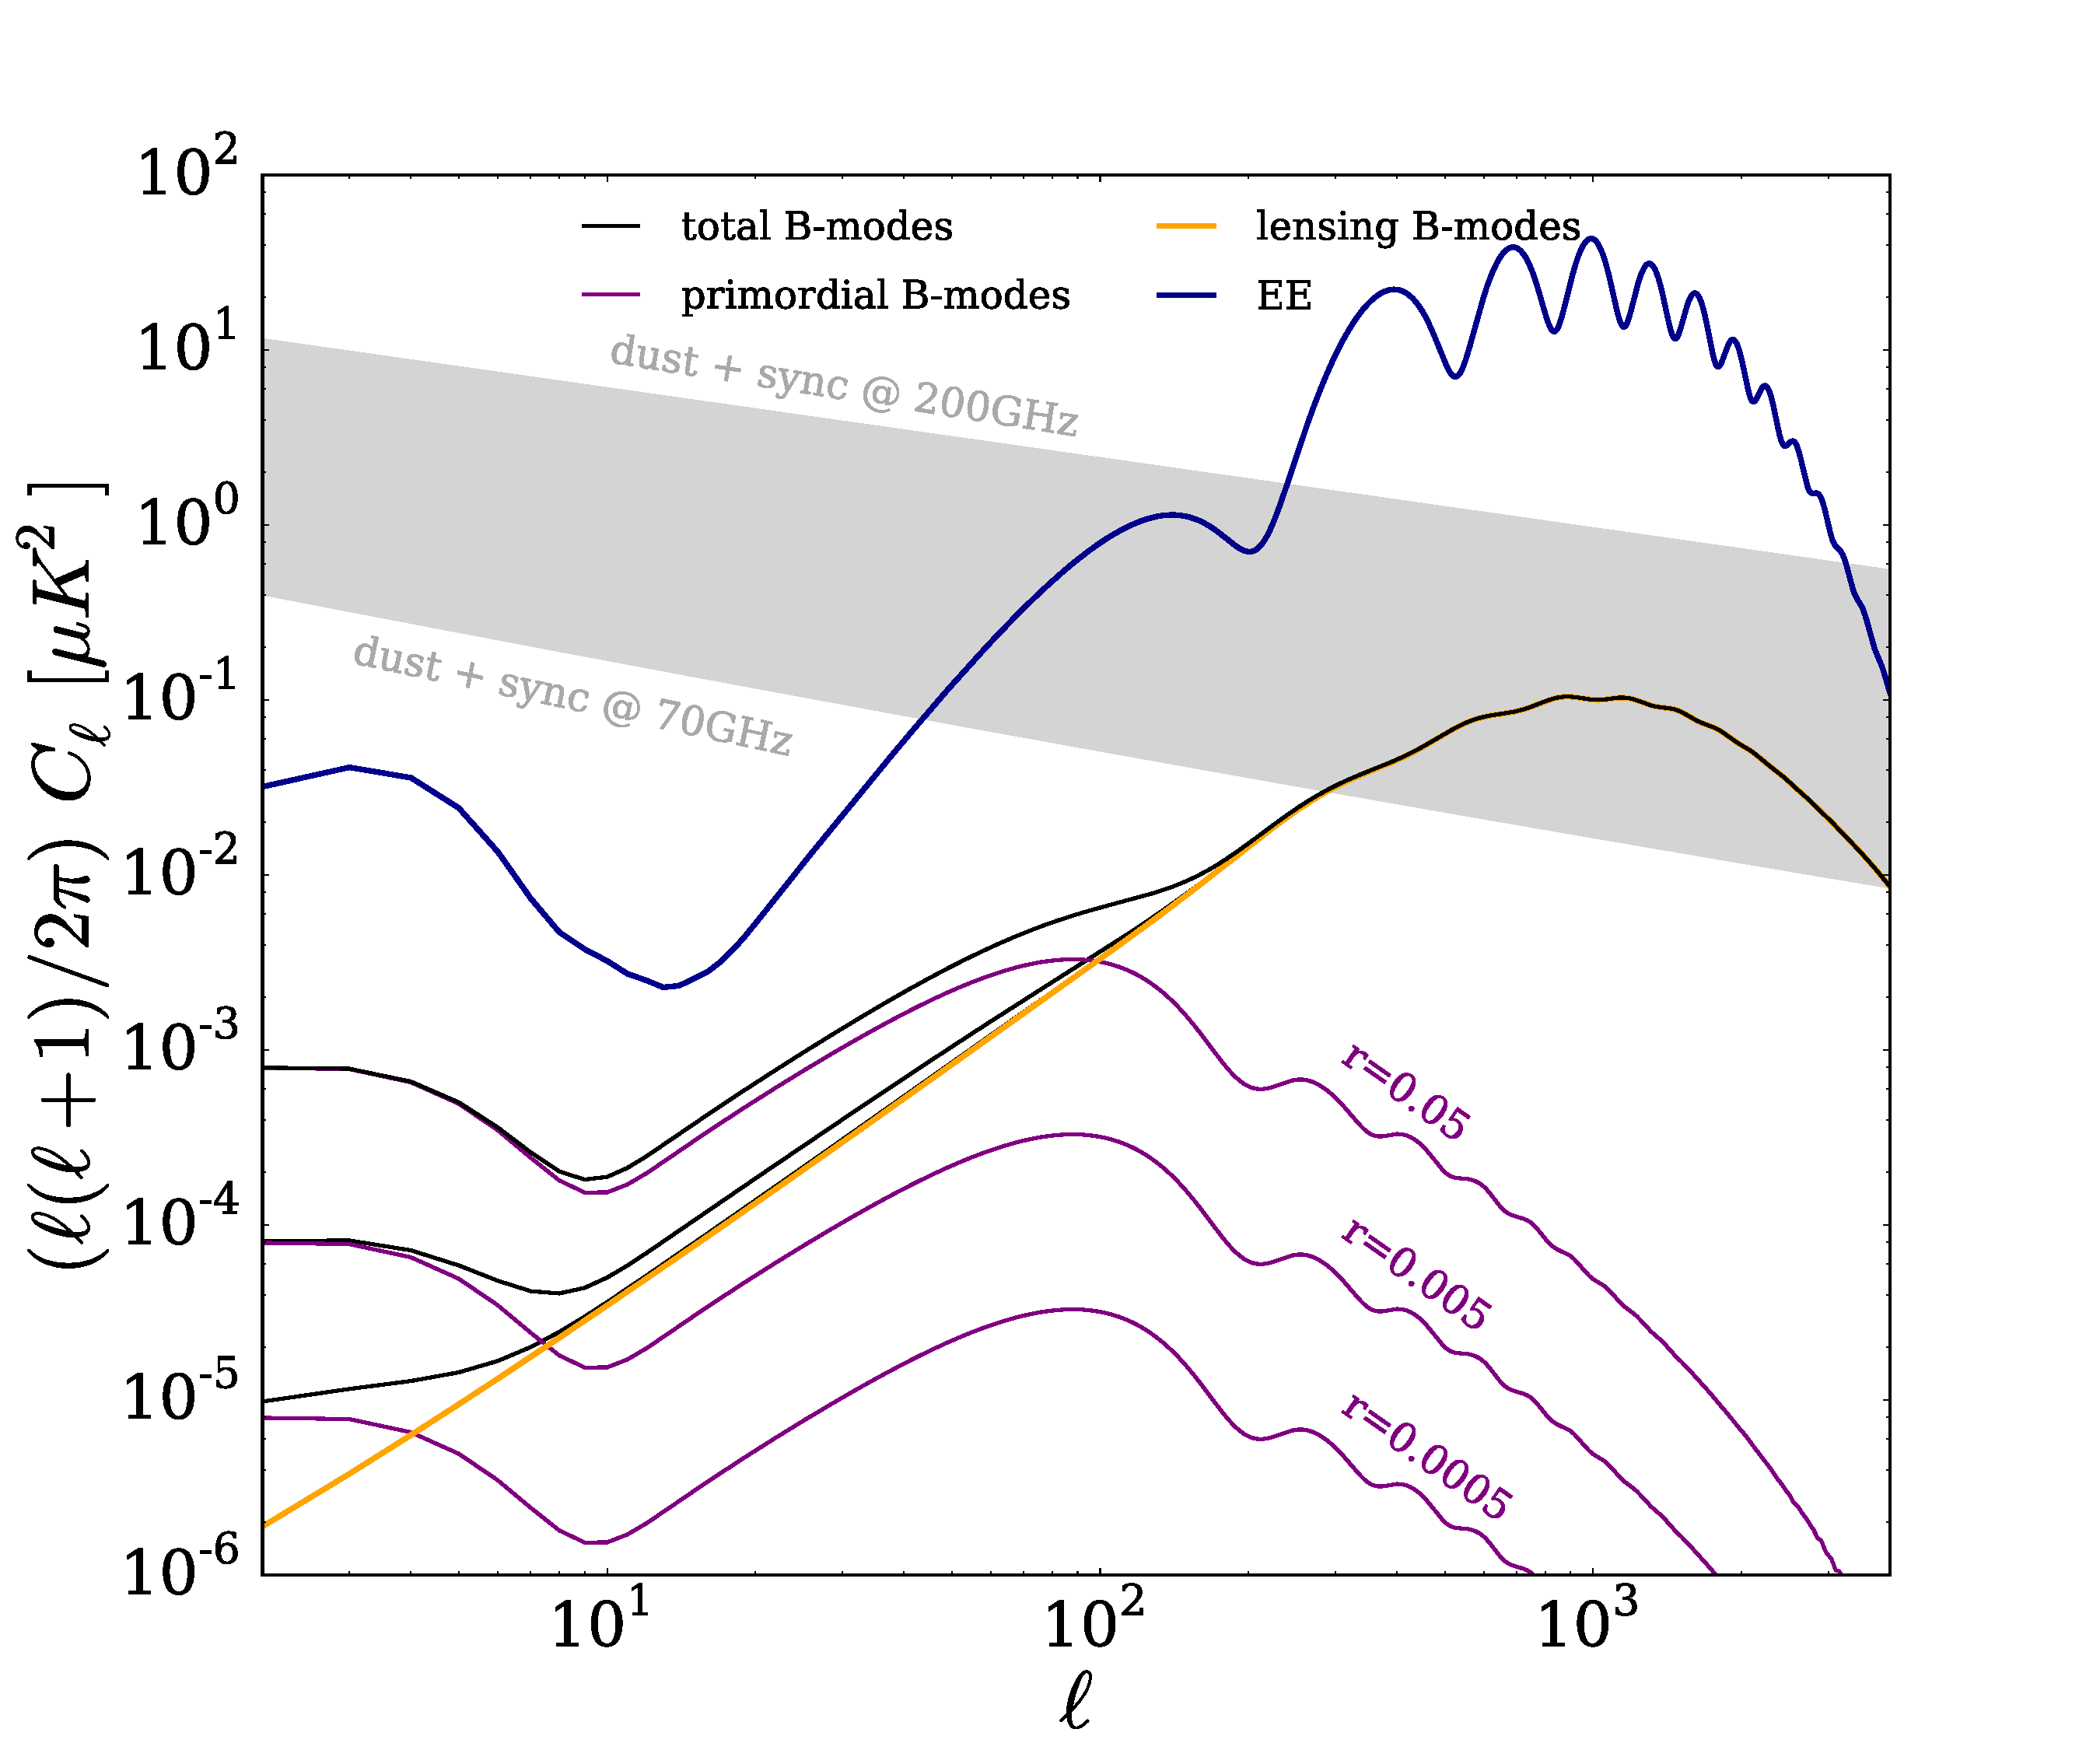
\includegraphics[width=3.12in]{Figures/clbb_freq_v2.pdf}
\end{center}
\caption{{\it Left panel:} Brightness temperature as function of frequency for the CMB as well as synchrotron emission (green) and dust emission (red). The darker bands show the brightness temperature for sky fractions between $73\%$ and $93\%$, the lighter bands show the brightness temperature for the cleanest $13\%$ with the width indicating the uncertainty. {\it Right panel:} Angular power spectrum for B-mode polarization of the CMB for $r=0.0005$, $r=0.005$, and $r=0.05$ as well as for foreground emission between 70 and 200 GHz.}
%, which shows the power spectrum of
%foregrounds over $75\%$ of the sky for frequencies between $70$ and
%$200$ GHz together with the lensing and inflationary contribution for
%different values of the tensor-to-scalar ratio.
\label{fig:frequency}
\end{figure}


One of the key ingredients in the design of a CMB experiment is the frequency coverage required to achieve the science goals. Consequently, optimizing frequency coverage in light of the new information from $Planck$ and its limitations will be one of key task of the study proposed here. 

%OVERVIEW of PLAN
To achieve these goals we plan a careful investigation of the effect on the measurements of r and $\tau$ of the presence of foreground residuals in the CMB maps (after foreground separation and/or cleaning) including, for example, the properties of the polarized thermal dust emission, specifically the spatial variation of its spectral index (hinted at by the observed decorrelation of the dust between 217 GHz and 353GHz Planck channels \ref{Planck2015-X;Planck2015-L;Planck2015-XXIX;Boulanger2016}), the breakdown of the modified black body spectrum model, and decorrelation between frequencies. 

These aspects will be explored with the help of physically motivated models of the foregrounds (\ref{Bruce+Fraisse2009,Hensley et al in preparation}) informed by existing data along with simulations based on these models. To incorporate instrument systematics due to beams, bandpass mismatches, correlated noise, etc., time domain based simulations will be required.

%INSTRUMENTAL PARAMETERS:
To devise the optimal instrumental/observational concept/design we will probe several configurations by varying critical instrumental parameters such as: the frequency coverage, the number of frequency channels, inter-band separation (limited by the typical instrumental bandwidths), the noise or sensitivity of each frequency channel, and angular resolution. 

%FG MODELLING:
Given that the B-mode signal is very weak, and much fainter than galactic foreground emission, even slight inacuracies in the characterization of the foregrounds will potentially impact the detectability of the B-mode signal. Therefore it is crucial to consider a large frequency coverage to properly gather the nature of the foregrounds as well as 'realistic' models that capture intrinsic complexities of these diffuse polarized foregrounds.
Therefore we will consider physically motivated dust models (beyond the modified blackbody spectrum approximation) currently in development. 
For these models the absorption cross-section in Intensity and Polarization are estimated self-consistently for grains of different sizes, shapes, and compositions as a function of frequency. These physical dust models will be used along with models implemented in the Planck Sky Model, PSM \ref{}, and/or  Python Sky model, PySm \ref{}, 


%TECHNIQUES:
To forecast the performance of a given instrumental design we will resort, for a quick diagnosis, to traditional techniques such as Fisher codes, both spectra and map based, that account for the presence of foregrounds assuming some best fit model of both the CMB and Foregrounds (akin to those used for the CMB-S4 science book \ref{}, eg CMB4cast (http://portal.nersc.gov/project/mp107/index.html)). 

%SIMULATIONS
For a more in depth analysis, that can also probe biases in the parameters, we will simulate maps of the CMB and Foreground emission at each frequency with CAMB and PSM (or PYSM) packages respectively and HEALpix modules \ref{}. Noise simulations will then be added to the signal maps.
While white noise or anisotropic noise are straightforwardly simulated directly on map domain, 1/f or correlated noise requires simulating time ordered data according to a noise prescription or generator (eg akin to LevelS \ref{} used in Planck). The convolution of the simulated maps with the Gaussian beams can be performed straightforwardly with HEALpix modules, while the convolution with more realistic beams is harder but can be performed with approaches such as FEBeCOP \ref{}, developed for Planck data analysis. To apply the latter an optical beam and scanning strategy needs to be specified and adopted by the software.

The next step is to clean the frequency maps from foregrounds and generate the 'clean' CMB map, using techniques such as Commander, SMICA, SEVEM and possibly NILC \ref{Planck2015-IX}. This is followed by estimation of auto and cross-correlation angular power spectra of the maps using say Master based \ref{}  or XFaster \ref{} based techniques and propagated to parameter estimation using CosmoMC or Multinest sampling.
Along with this standard procedure we will also apply a novel technique based on direct Bayesian MCMC inference of cosmological parameters in the presence of foregrounds, without resorting to Likelihood approximations (an extension of the method presented in  \ref{Jewelletal2016}). 
The latter will be integrated with Commander, allowing to bypass the angular power spectrum estimation as it samples Cosmological and Foregrounds parameters directly from the simulated maps. As in this approach the foreground parameter fits (including the spectral index) is performed pixel by pixel, the spatial variation of the spectral index is naturally accounted for. 

%As mentioned earlier 1/f or correlated noise requires simulating time ordered data. To analyse the resulting maps another ingredient is needed, the pixel-to-pixel noise correlation matrix. For a large number of pixels the estimation of this matrix is computationally intensive. As 1/f and correlated noise leaves mostly in the large angular scales and we resort to studying these effects on low resolution maps (reducing computational costs), hybridized with higher resolution maps for the white noise component. 

It should be stressed that to fully assess the performance of a given instrument design, in view of both foreground residuals and the presence of systematics, realistic simulations are essential. These include time domain based simulations which can be generated using HPC4CMB ((https://github.com/hpc4cmb)) based on TOAST 
%(data framework, including on-the-fly simulation capabilities with full detector beam, bandpass and noise properties)), 
and a destriper based map-making algorithm such as libMADAM. 


%FOM
Finally to quantify performance we will need to define a figure of merit, FOM. Examples of possible FOM, are: the effective noise in the I,Q,U maps after foreground cleaning (effectively quantifying the noise degradation due to the presence of residual foregrounds); uncertainty and biases in the parameters; the evidence of the best fit model for each instrumental design (used as a qualifier of the instrumental design itself), etc.


\comred{GR:This is a first version of the plan - still needs editing} 
 



%references
%Bruce+Fraisse2009 - 2009ApJ...696....1D
%Planck2015-IX - 2016A&A...594A...9P
%Planck2015-X - 2016A&A...594A..10P
%Planck2015-XXIX - A&A 586, A132 (2016)
%Planck2015-L - arXiv:1606.07335v1;
%Boulanger2016 - A&A 580, A136 (2015)
%Jewell2016 -  ApJ., 820, 2016
%





% Raphael, Josquin, Aurelien, Charles, Graca
